% Created by tikzDevice version 0.12.3.1 on 2021-11-19 20:56:52
% !TEX encoding = UTF-8 Unicode
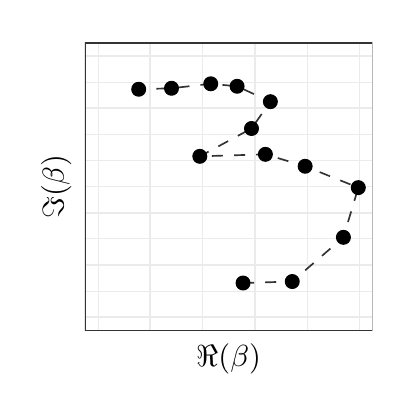
\begin{tikzpicture}[x=1pt,y=1pt]
\definecolor{fillColor}{RGB}{255,255,255}
\path[use as bounding box,fill=fillColor,fill opacity=0.00] (0,0) rectangle (130.09,130.09);
\begin{scope}
\path[clip] (  0.00,  0.00) rectangle (130.09,130.09);
\definecolor{drawColor}{RGB}{255,255,255}
\definecolor{fillColor}{RGB}{255,255,255}

\path[draw=drawColor,line width= 0.6pt,line join=round,line cap=round,fill=fillColor] (  0.00,  0.00) rectangle (130.09,130.09);
\end{scope}
\begin{scope}
\path[clip] ( 20.71, 20.71) rectangle (124.59,124.59);
\definecolor{fillColor}{RGB}{255,255,255}

\path[fill=fillColor] ( 20.71, 20.71) rectangle (124.59,124.59);
\definecolor{drawColor}{gray}{0.92}

\path[draw=drawColor,line width= 0.3pt,line join=round] ( 20.71, 34.88) --
	(124.59, 34.88);

\path[draw=drawColor,line width= 0.3pt,line join=round] ( 20.71, 53.76) --
	(124.59, 53.76);

\path[draw=drawColor,line width= 0.3pt,line join=round] ( 20.71, 72.65) --
	(124.59, 72.65);

\path[draw=drawColor,line width= 0.3pt,line join=round] ( 20.71, 91.54) --
	(124.59, 91.54);

\path[draw=drawColor,line width= 0.3pt,line join=round] ( 20.71,110.42) --
	(124.59,110.42);

\path[draw=drawColor,line width= 0.3pt,line join=round] ( 25.44, 20.71) --
	( 25.44,124.59);

\path[draw=drawColor,line width= 0.3pt,line join=round] ( 63.21, 20.71) --
	( 63.21,124.59);

\path[draw=drawColor,line width= 0.3pt,line join=round] (100.98, 20.71) --
	(100.98,124.59);

\path[draw=drawColor,line width= 0.6pt,line join=round] ( 20.71, 25.44) --
	(124.59, 25.44);

\path[draw=drawColor,line width= 0.6pt,line join=round] ( 20.71, 44.32) --
	(124.59, 44.32);

\path[draw=drawColor,line width= 0.6pt,line join=round] ( 20.71, 63.21) --
	(124.59, 63.21);

\path[draw=drawColor,line width= 0.6pt,line join=round] ( 20.71, 82.09) --
	(124.59, 82.09);

\path[draw=drawColor,line width= 0.6pt,line join=round] ( 20.71,100.98) --
	(124.59,100.98);

\path[draw=drawColor,line width= 0.6pt,line join=round] ( 20.71,119.86) --
	(124.59,119.86);

\path[draw=drawColor,line width= 0.6pt,line join=round] ( 44.32, 20.71) --
	( 44.32,124.59);

\path[draw=drawColor,line width= 0.6pt,line join=round] ( 82.09, 20.71) --
	( 82.09,124.59);

\path[draw=drawColor,line width= 0.6pt,line join=round] (119.86, 20.71) --
	(119.86,124.59);
\definecolor{drawColor}{RGB}{0,0,0}

\path[draw=drawColor,draw opacity=0.80,line width= 0.6pt,dash pattern=on 4pt off 4pt ,line join=round] ( 77.82, 37.82) --
	( 95.60, 38.36) --
	(114.09, 54.33) --
	(119.47, 72.29) --
	(100.26, 80.01) --
	( 85.90, 84.32) --
	( 62.20, 83.60) --
	( 80.88, 93.65) --
	( 87.70,103.35) --
	( 75.67,108.91) --
	( 66.15,109.81) --
	( 51.97,108.19) --
	( 40.12,107.84);
\definecolor{drawColor}{RGB}{0,0,0}
\definecolor{fillColor}{RGB}{0,0,0}

\path[draw=drawColor,line width= 0.4pt,line join=round,line cap=round,fill=fillColor] ( 77.82, 37.82) circle (  2.50);

\path[draw=drawColor,line width= 0.4pt,line join=round,line cap=round,fill=fillColor] ( 95.60, 38.36) circle (  2.50);

\path[draw=drawColor,line width= 0.4pt,line join=round,line cap=round,fill=fillColor] (114.09, 54.33) circle (  2.50);

\path[draw=drawColor,line width= 0.4pt,line join=round,line cap=round,fill=fillColor] (119.47, 72.29) circle (  2.50);

\path[draw=drawColor,line width= 0.4pt,line join=round,line cap=round,fill=fillColor] (100.26, 80.01) circle (  2.50);

\path[draw=drawColor,line width= 0.4pt,line join=round,line cap=round,fill=fillColor] ( 85.90, 84.32) circle (  2.50);

\path[draw=drawColor,line width= 0.4pt,line join=round,line cap=round,fill=fillColor] ( 62.20, 83.60) circle (  2.50);

\path[draw=drawColor,line width= 0.4pt,line join=round,line cap=round,fill=fillColor] ( 80.88, 93.65) circle (  2.50);

\path[draw=drawColor,line width= 0.4pt,line join=round,line cap=round,fill=fillColor] ( 87.70,103.35) circle (  2.50);

\path[draw=drawColor,line width= 0.4pt,line join=round,line cap=round,fill=fillColor] ( 75.67,108.91) circle (  2.50);

\path[draw=drawColor,line width= 0.4pt,line join=round,line cap=round,fill=fillColor] ( 66.15,109.81) circle (  2.50);

\path[draw=drawColor,line width= 0.4pt,line join=round,line cap=round,fill=fillColor] ( 51.97,108.19) circle (  2.50);

\path[draw=drawColor,line width= 0.4pt,line join=round,line cap=round,fill=fillColor] ( 40.12,107.84) circle (  2.50);
\definecolor{drawColor}{gray}{0.20}

\path[draw=drawColor,line width= 0.6pt,line join=round,line cap=round] ( 20.71, 20.71) rectangle (124.59,124.59);
\end{scope}
\begin{scope}
\path[clip] (  0.00,  0.00) rectangle (130.09,130.09);
\definecolor{drawColor}{RGB}{0,0,0}

\node[text=drawColor,anchor=base,inner sep=0pt, outer sep=0pt, scale=  1.10] at ( 72.65,  7.64) {$\Re(\beta)$};
\end{scope}
\begin{scope}
\path[clip] (  0.00,  0.00) rectangle (130.09,130.09);
\definecolor{drawColor}{RGB}{0,0,0}

\node[text=drawColor,rotate= 90.00,anchor=base,inner sep=0pt, outer sep=0pt, scale=  1.10] at ( 13.08, 72.65) {$\Im(\beta)$};
\end{scope}
\end{tikzpicture}
